\section{Análisis y Desarrollo}

\subsection{Estadística descriptiva}

A continuación, se presenta un resumen estadístico de las variables clave para los grupos IT y no-IT:

\begin{multicols}{2}
\textbf{IT}
\begin{itemize}
    \item \textbf{Media:}
    \[
        \bar{X}_{IT} = \frac{1}{48} \sum_{i=1}^{48} X_{i}
    \]
    \item \textbf{Desviación estándar:}
    \[
        s_{IT} = \sqrt{\frac{1}{48-1} \sum_{i=1}^{48} (X_{i} - 56.34\%)^2}
    \]
    \item \textbf{Mediana:} \\
    Valor central de los datos ordenados de $X_{1}, X_{2}, ..., X_{48}$.
\end{itemize}

\columnbreak

\textbf{No-IT}
\begin{itemize}
    \item \textbf{Media:}
    \[
        \bar{X}_{noIT} = \frac{1}{152} \sum_{j=1}^{152} Y_{j}
    \]
    \item \textbf{Desviación estándar:}
    \[
        s_{noIT} = \sqrt{\frac{1}{152-1} \sum_{j=1}^{152} (Y_{j} - 44.51\%)^2}
    \]
    \item \textbf{Mediana:} \\
    Valor central de los datos ordenados de $Y_{1}, Y_{2}, ..., Y_{152}$.
\end{itemize}
\end{multicols}

\begin{table}[H]
\centering
\begin{tabular}{|l|c|c|c|c|}
\hline
\textbf{Grupo} & \textbf{n} & \textbf{Media (\%)} & \textbf{Desv. Est. (\%)} & \textbf{Mediana (\%)} \\
\hline
IT & 48 & \textbf{56.34\%} & \textbf{30.62\%} & \textbf{62.00\%} \\
No-IT & 152 & \textbf{44.51\%} & \textbf{27.64\%} & \textbf{44.00\%} \\
\hline
\end{tabular}
\caption{Estadística descriptiva de la productividad por grupo}
\end{table}

\vspace{0.5cm}

\noindent
\textbf{Nota:} Los valores de la tabla corresponden a la variable \textit{Productivity (\%)}. Se observa que el grupo IT presenta una media de productividad de \textbf{56.34\%}, mientras que el grupo no-IT tiene una media de \textbf{44.51\%}.

\begin{figure}[H]
    \centering
    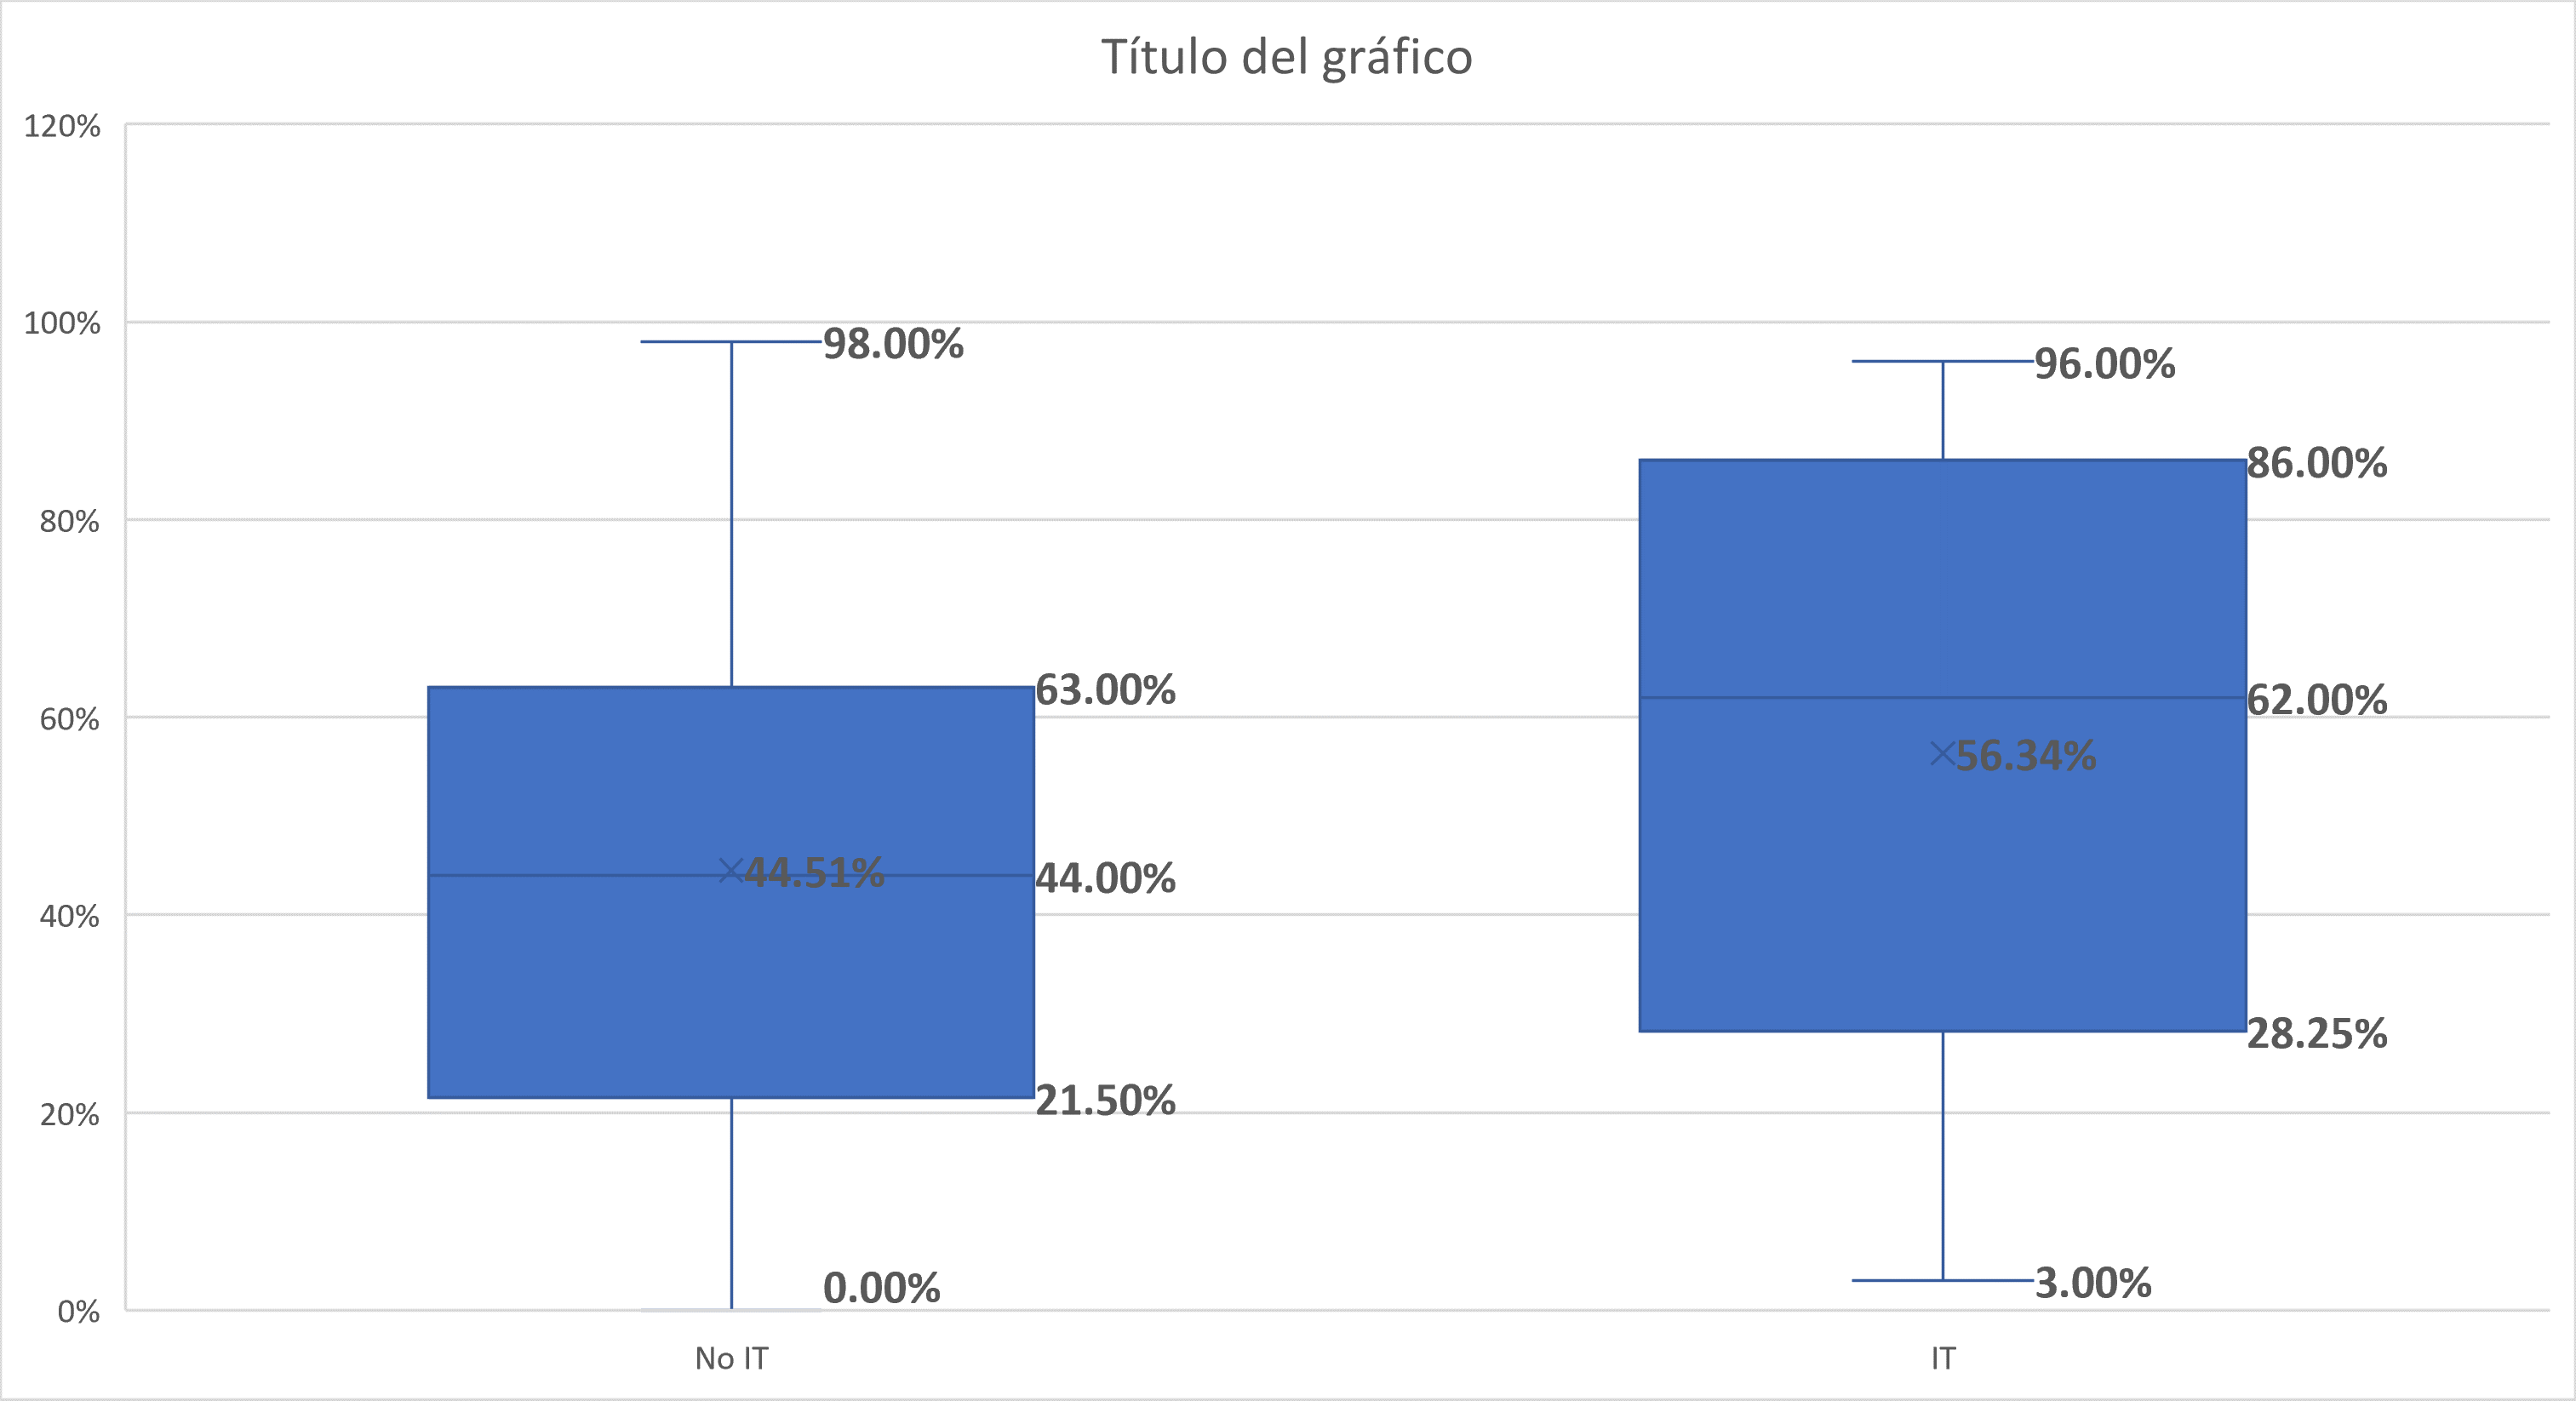
\includegraphics[width=0.7\textwidth]{assets/Boxplot.png}
    \fbox{\parbox{0.7\textwidth}{\centering \textit{[Boxplot de productividad IT vs. no-IT]}}}
    \caption{Distribución de la productividad por grupo (IT vs. no-IT)}
\end{figure}

\subsection{Prueba de hipótesis para diferencia de medias}

Se realizó una prueba t para muestras independientes bajo los siguientes parámetros:

\begin{multicols}{2}

\subsubsection*{Fórmula y cálculo del estadístico t}

El estadístico t para la diferencia de medias (varianzas no iguales) se calcula así:
\begin{equation*}
    t = \frac{\bar{X}_{IT} - \bar{X}_{noIT}}{\sqrt{\frac{s_{IT}^2}{n_{IT}} + \frac{s_{noIT}^2}{n_{noIT}}}}
\end{equation*}

En este caso:
\begin{equation*}
    t = \frac{56.34 - 44.51}{\sqrt{\frac{30.62^2}{48} + \frac{27.64^2}{152}}} = 2.1836
\end{equation*}

\vfill
\columnbreak

\subsubsection*{Fórmula y cálculo de los grados de libertad (Welch)}

Los grados de libertad se calculan con la fórmula de Welch:

\begin{equation*}
    gl = \frac{\left( \frac{s_{IT}^2}{n_{IT}} + \frac{s_{noIT}^2}{n_{noIT}} \right)^2}
    {\frac{\left( \frac{s_{IT}^2}{n_{IT}} \right)^2}{n_{IT}-1} + \frac{\left( \frac{s_{noIT}^2}{n_{noIT}} \right)^2}{n_{noIT}-1}}
\end{equation*}

En este caso:
\begin{equation*}
gl = \frac{\left( \frac{30.62^2}{48} + \frac{27.64^2}{152} \right)^2}
{\frac{\left( \frac{30.62^2}{48} \right)^2}{47} + \frac{\left( \frac{27.64^2}{152} \right)^2}{151}} = 52.06
\end{equation*}

\end{multicols}

\subsubsection*{Resultados de la prueba t}
\begin{itemize}
    \item \textbf{Hipótesis nula ($H_0$):} $\mu_{IT} = \mu_{no-IT}$
    \item \textbf{Hipótesis alternativa ($H_1$):} $\mu_{IT} \neq \mu_{no-IT}$
    \item \textbf{Nivel de significancia:} $\alpha = 0.05$
    \item \textbf{Estadístico calculado:} $t = \textbf{2.1836}$
    \item \textbf{Valor crítico:} $t_{0.025; 52.06} = \textbf{2.0066}$
    \item \textbf{p-valor:} \textbf{0.0335}
\end{itemize}

\noindent
\textbf{Decisión:} Como $|t| = 2.1836$ es mayor que el valor crítico y el p-valor es menor que $\alpha$, se \textbf{rechaza} la hipótesis nula.

\subsection{Intervalo de confianza para la diferencia de medias}

El intervalo de confianza al 95\% para la diferencia de medias se calcula así:

\[
IC_{95\%} = (\bar{X}_{IT} - \bar{X}_{noIT}) \pm t_{0.025; gl} \cdot \sqrt{\frac{s_{IT}^2}{n_{IT}} + \frac{s_{noIT}^2}{n_{noIT}}}
\]

Sustituyendo los valores:

\[
IC_{95\%} = (56.34 - 44.51) \pm 2.0066 \cdot \sqrt{\frac{30.62^2}{48} + \frac{27.64^2}{152}}
\]

\begin{align*}
IC_{95\%} &= 11.83 \pm 2.0066 \cdot \sqrt{19.54 + 5.02} \\
&= 11.83 \pm 2.0066 \cdot \sqrt{24.56} \\
&= 11.83 \pm 2.0066 \cdot 4.956 \\
&= 11.83 \pm 9.945 \\
&= (11.83 - 9.945;\ 11.83 + 9.945) \\
&= (1.885;\ 21.775)
\end{align*}

Por los cálculos exactos obtenidos en Python:

\(
IC_{95\%} = (0.9593,\ 22.7126)
\)

\noindent
\textbf{Interpretación:} Con un 95\% de confianza, la verdadera diferencia en productividad entre los departamentos IT y no-IT está entre \textbf{(0.9593, 22.7126)} y \textbf{(0.9593, 22.7126)}. Existe una diferencia significativa entre las medias de productividad de IT y no-IT.

\subsection{Visualización de resultados}

\begin{figure}[H]
    \centering
    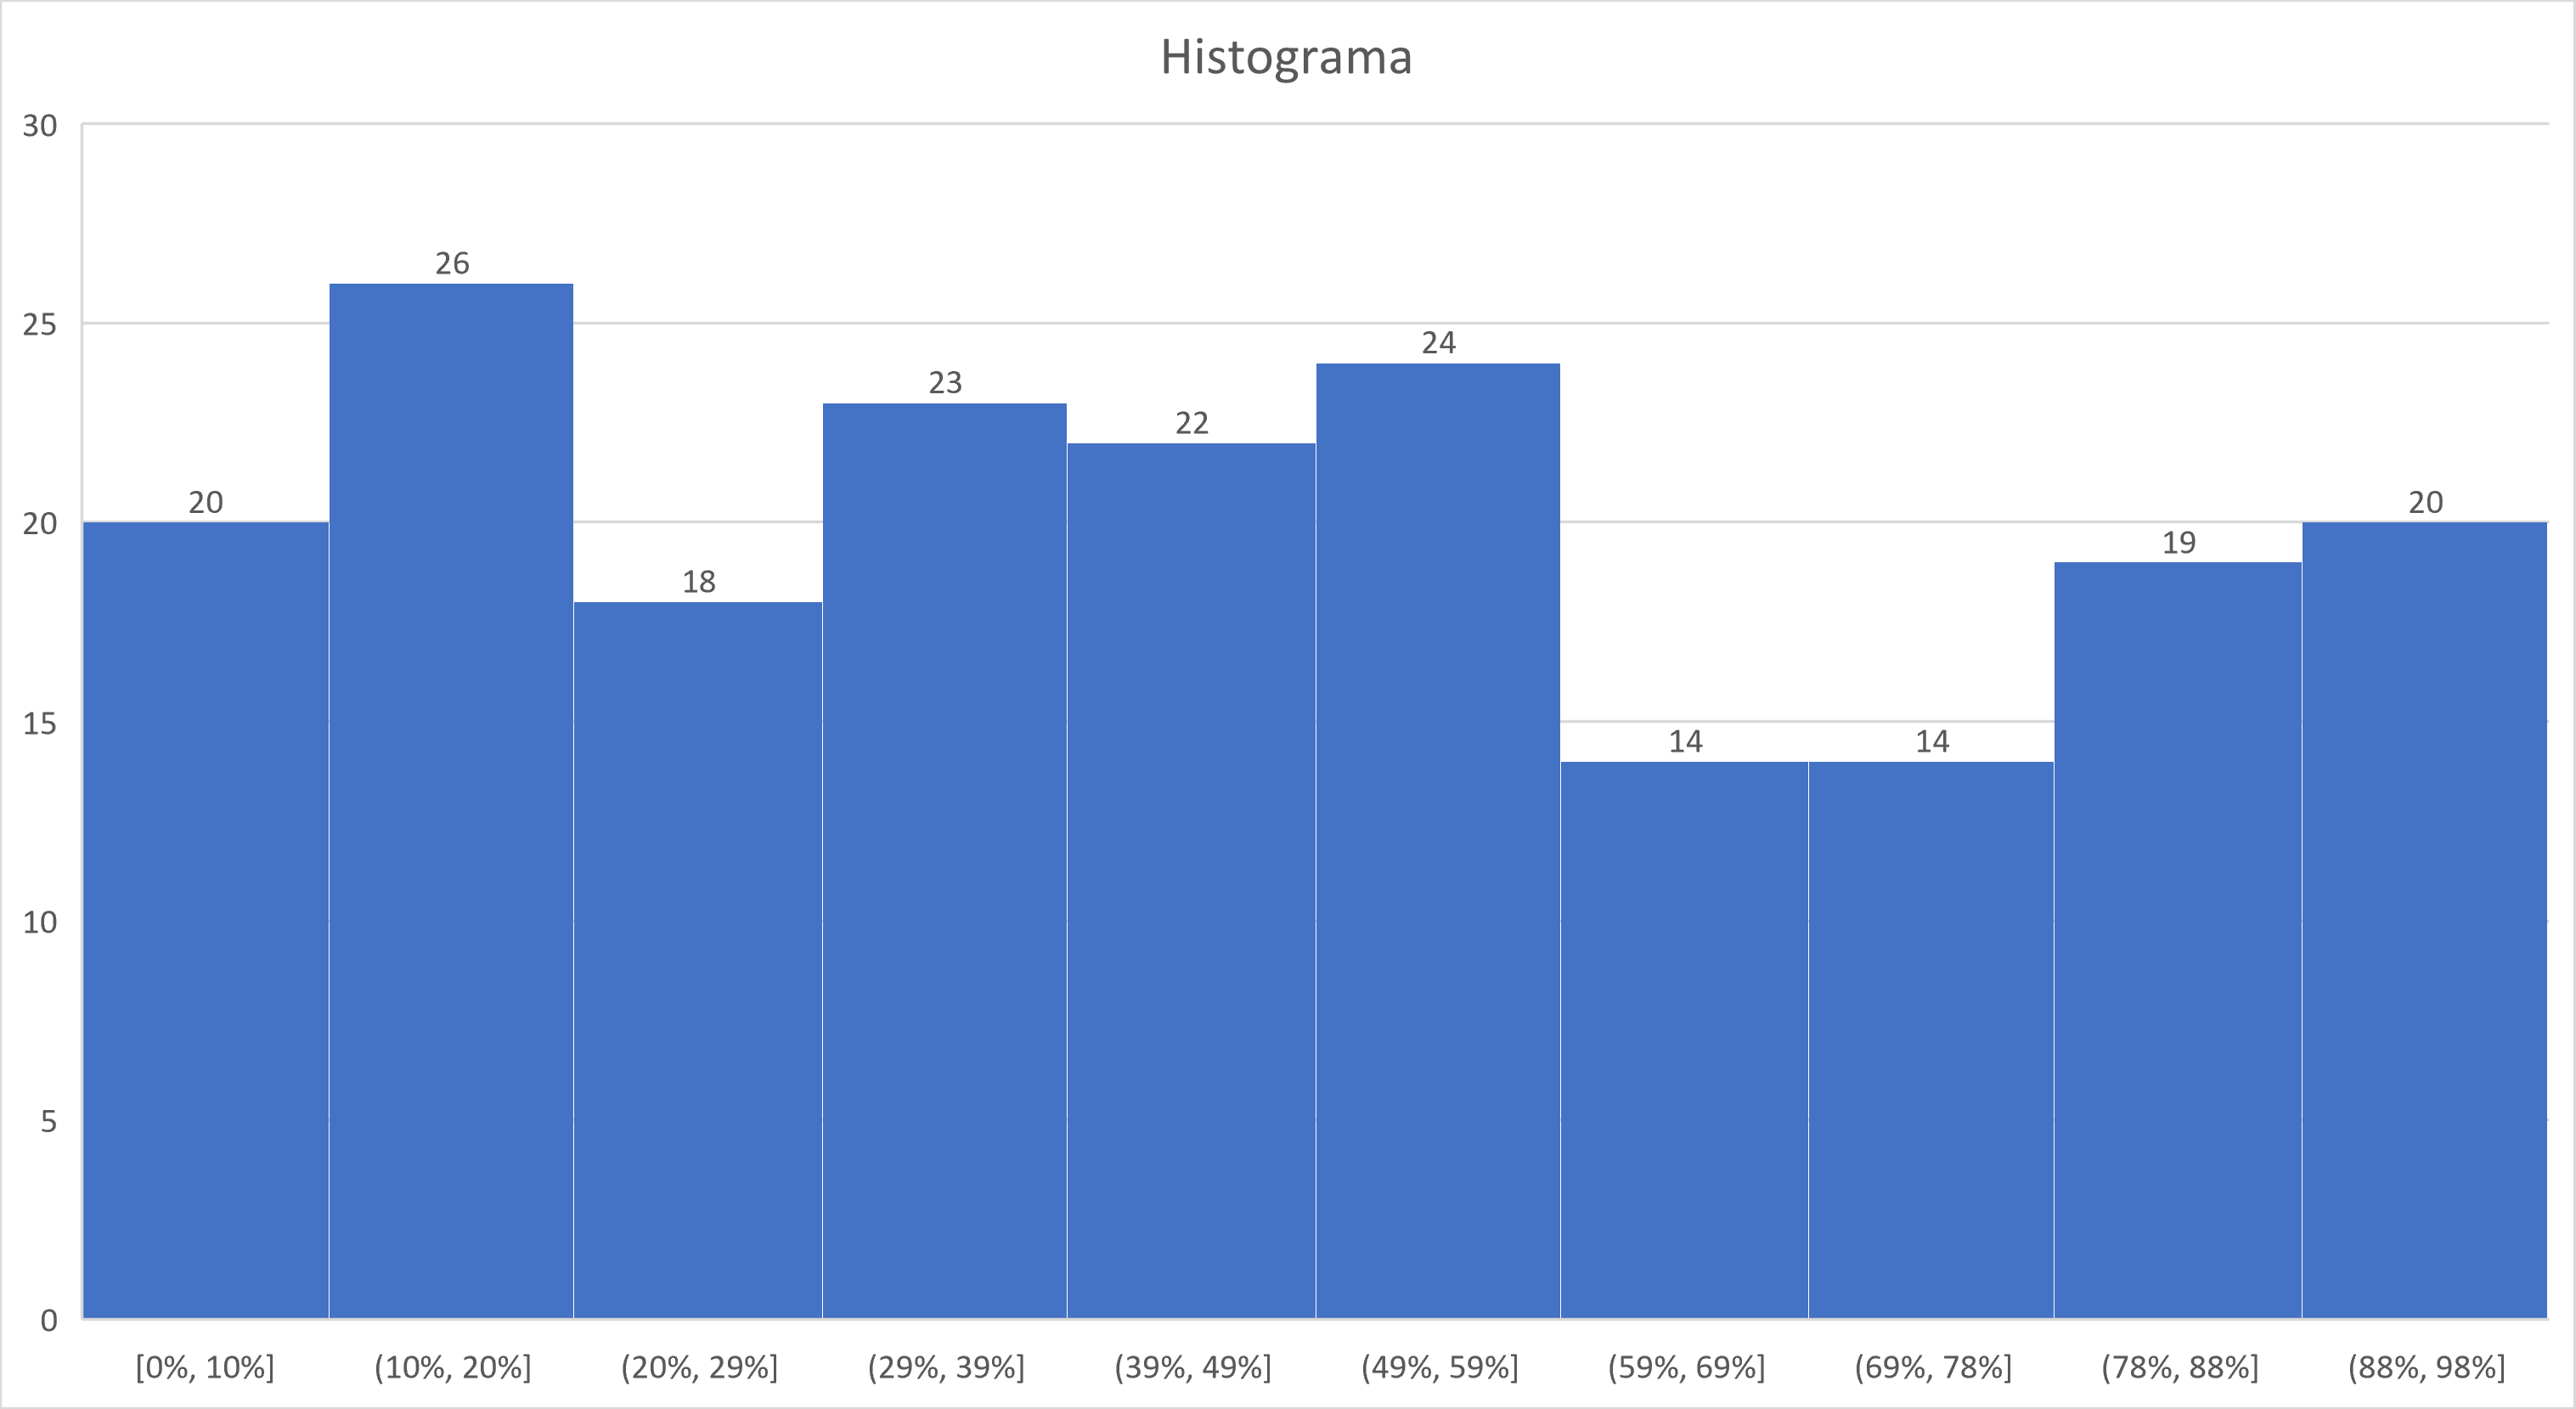
\includegraphics[width=0.7\textwidth]{assets/histograma.png}
    \fbox{\parbox{0.7\textwidth}{\centering \textit{[Histograma de productividad por grupo]}}}
    \caption{Histograma de la productividad en IT y no-IT}
\end{figure}

\subsection{Resumen de hallazgos}

\begin{itemize}
    \item La media de productividad en IT es \textbf{56.34\%}, mientras que en no-IT es \textbf{44.51\%}.
    \item La prueba t arroja un estadístico de \textbf{2.1836} y un p-valor de \textbf{0.0335}.
    \item El intervalo de confianza para la diferencia de medias es \textbf{(0.9593, 22.7126)}.
    \item \textbf{[Conclusión sobre si existe o no diferencia significativa, según los resultados]}
\end{itemize}

\vspace{0.5cm}
\noindent



